\lecture{3}{2025-09-23}{oui}{}
\subsection{Fin de l'impact de l'énergie sur la société}

\begin{parag}{Effet Rebond}
    \begin{definition}
        En trouvant une solution au problème la solution finalement empire ce problème
    \end{definition}
    \begin{subparag}{Exemple}
        Par exemple, vouloir manger moins de calorie en mangant de la glace basse en calorie mais ducoup en manger plus car moins calorique $\to$ plus de calorie au final.
    \end{subparag}
\end{parag}
\begin{parag}{Evolution de la consommation finale d'energie}
	\begin{center}
    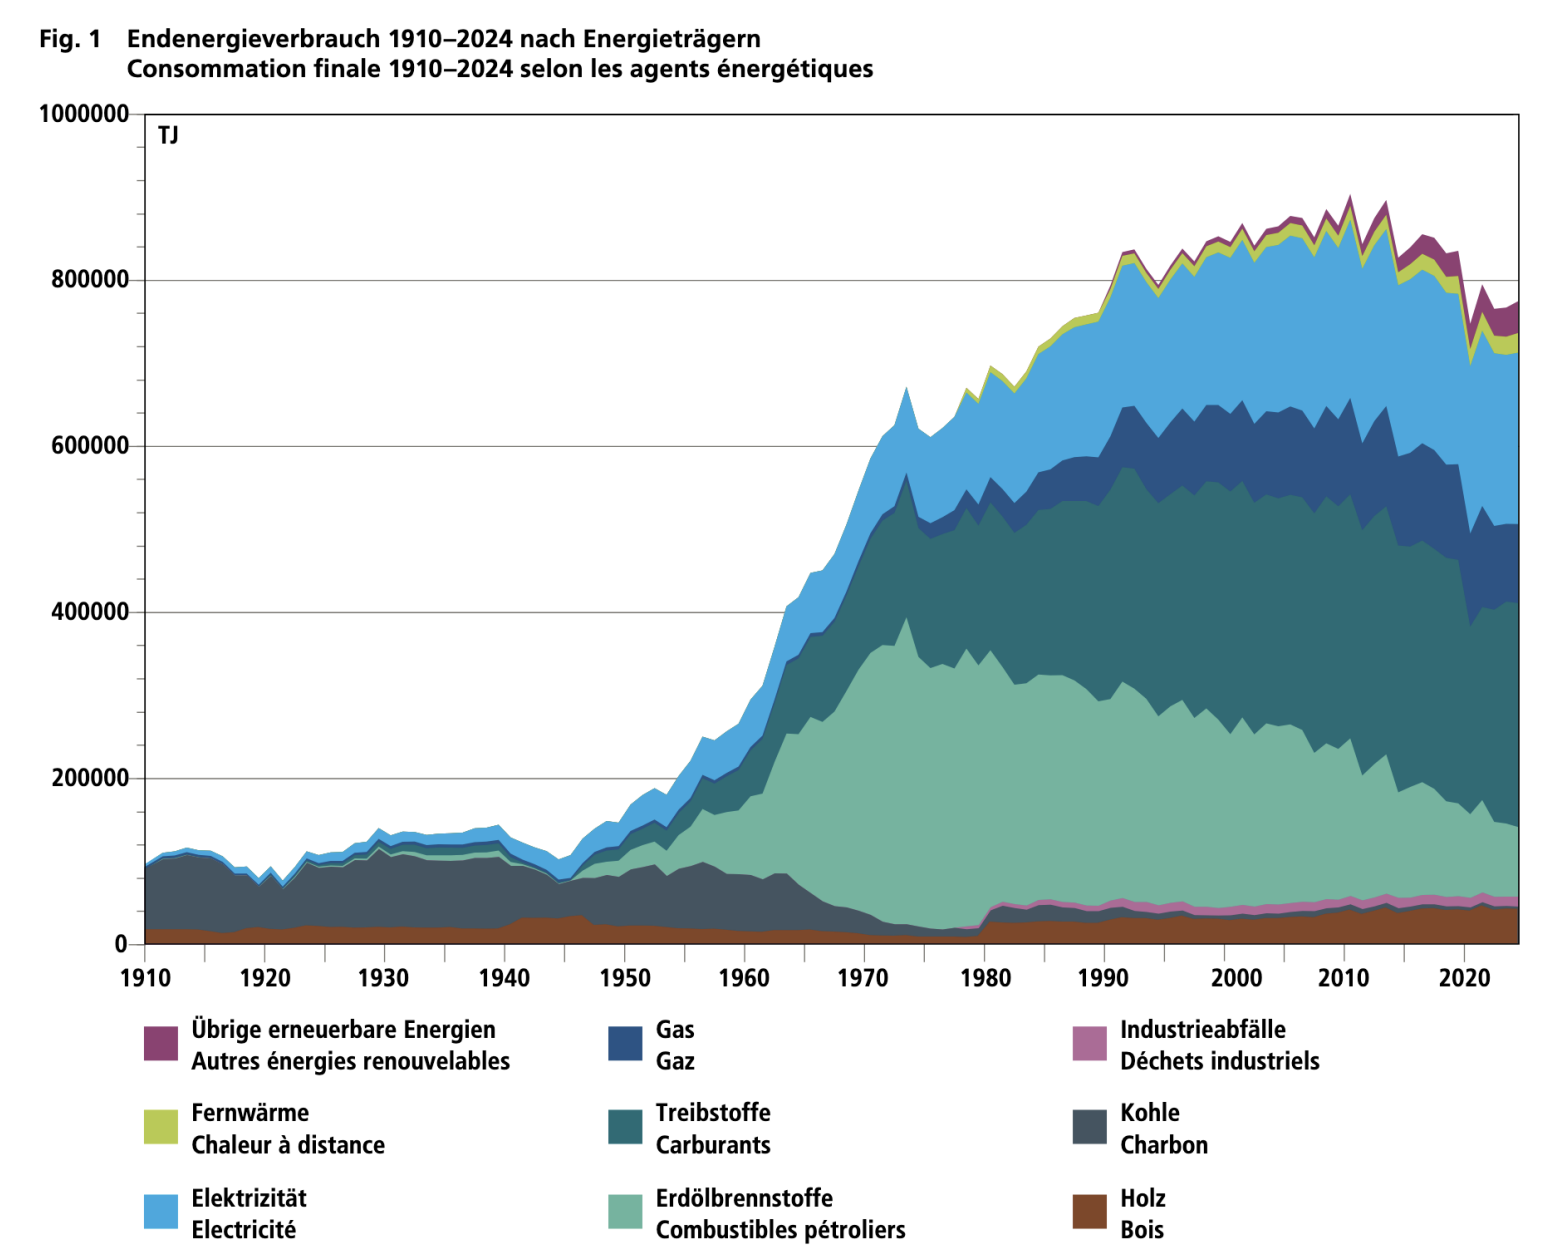
\includegraphics[scale=0.2]{12025-09-23.png}
	\end{center}
	
    On voit ici que cet emmissions est seulement au niveau locale (production sur le terrain Suisse) néanmoins beaucoup de la production est délocalisé de nos jours ce qui expliquer pourquoi la production peut baisser.
\end{parag}
\begin{parag}{Energie primaire, secondaire, finale, utile}

	\begin{center}
   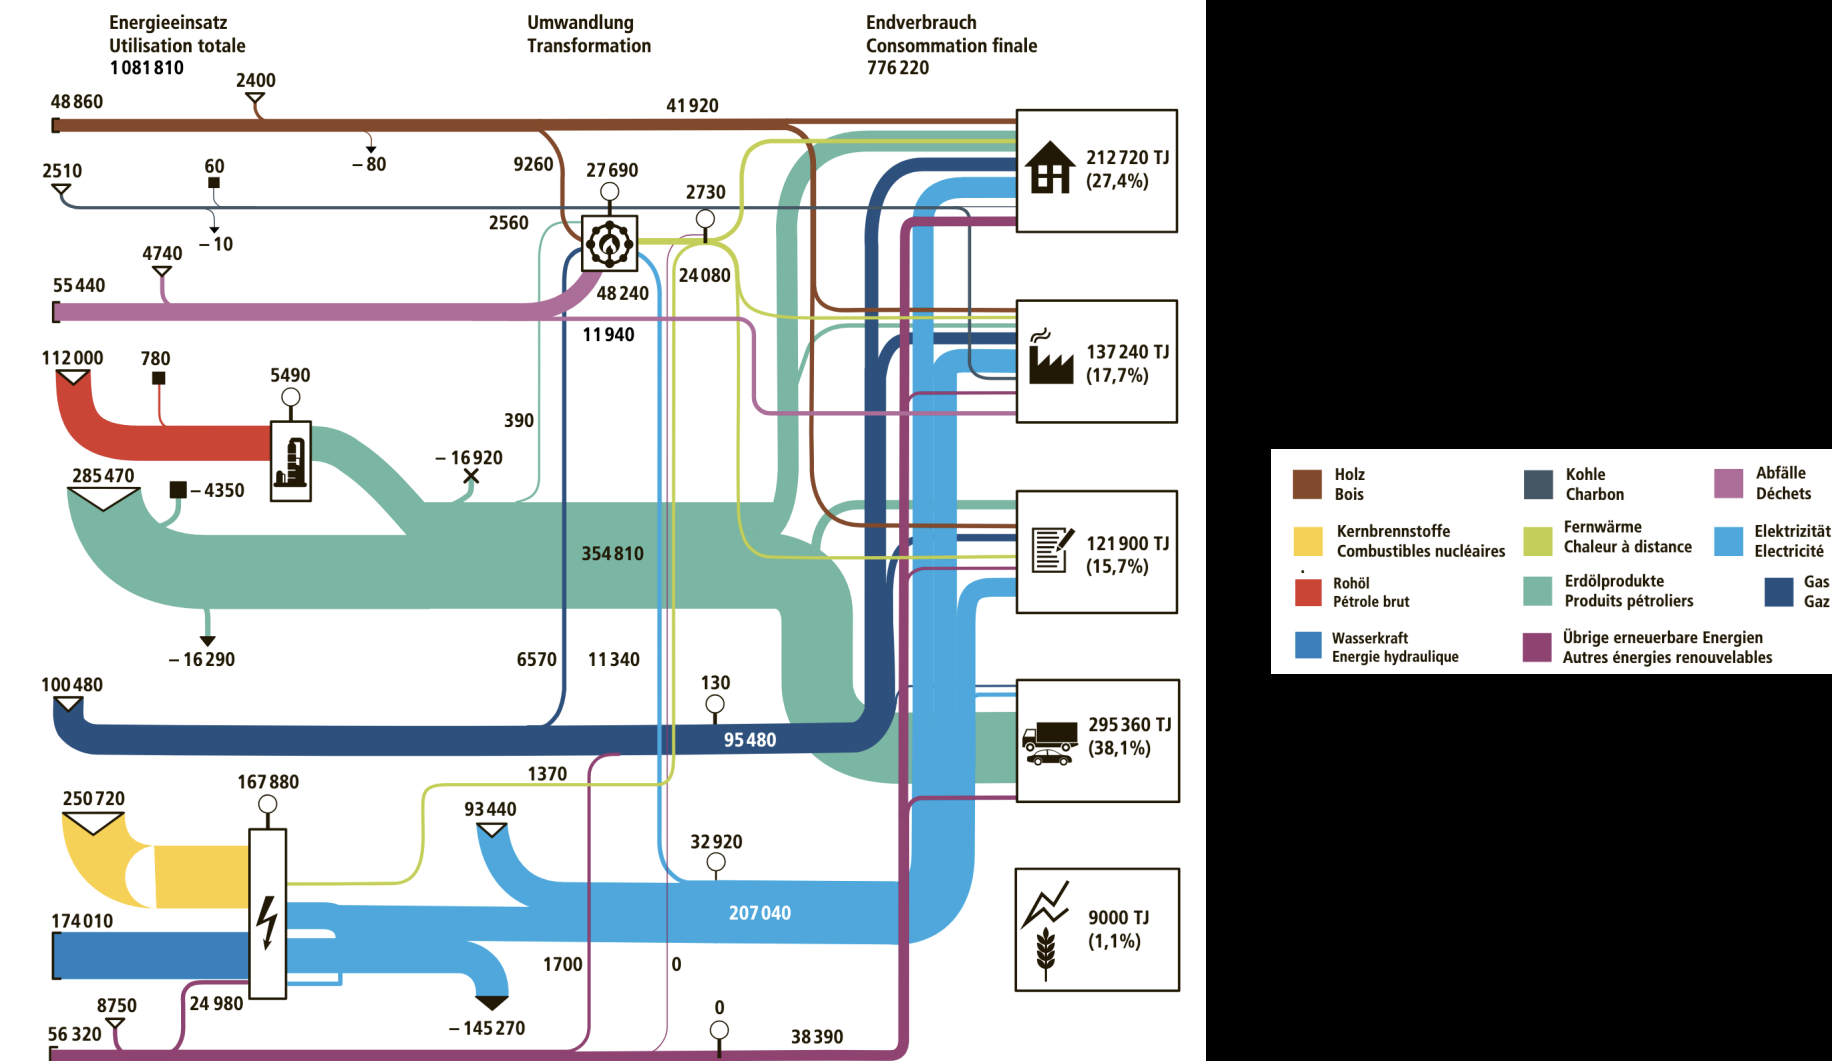
\includegraphics[scale=0.2]{22025-09-23.png} 
	\end{center}
	
\end{parag}



\begin{parag}{Pourquoi continue t-on à chercher?}
	\begin{center}
	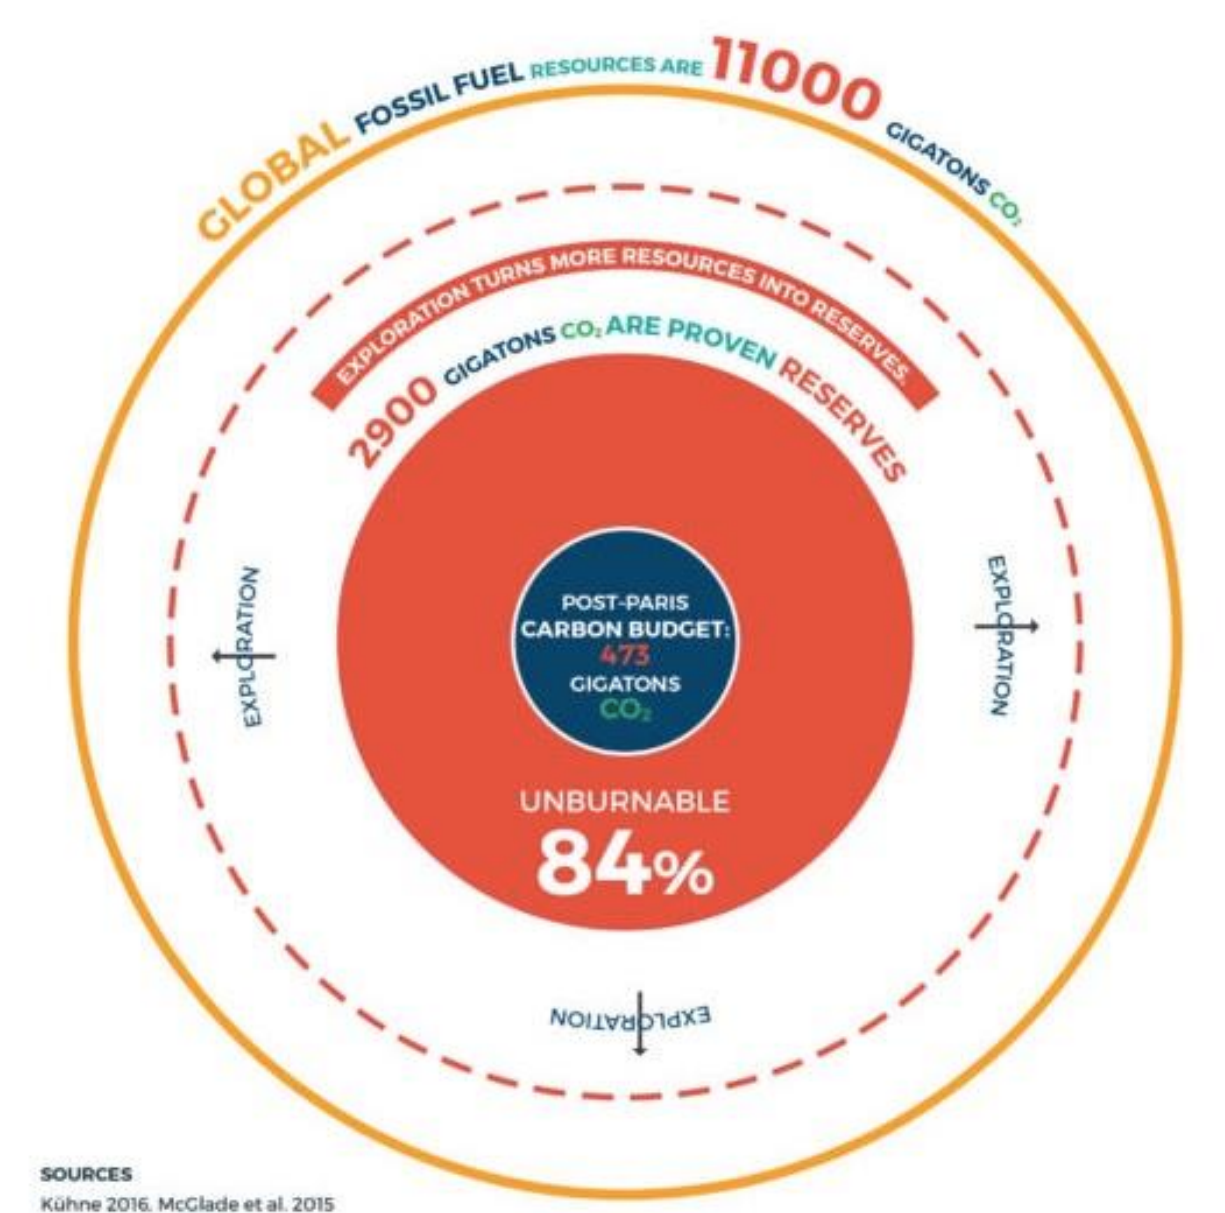
\includegraphics[scale=0.2]{42025-09-23.png}
	\end{center}
	
    Donc ici par rapport aux accord de paris (au maximum 2 degrés de réchauffement). Si on brûle toute la reserve de pétrole qu'on a, il y en a 84\% qui sont en surplus\\
    Ici ce qui est important c'est pas vraimment le stock mais plus le \important{flux}

\end{parag}
\begin{parag}{EROI des dlcouvertes (aux USA)}
	\begin{center}
	    
	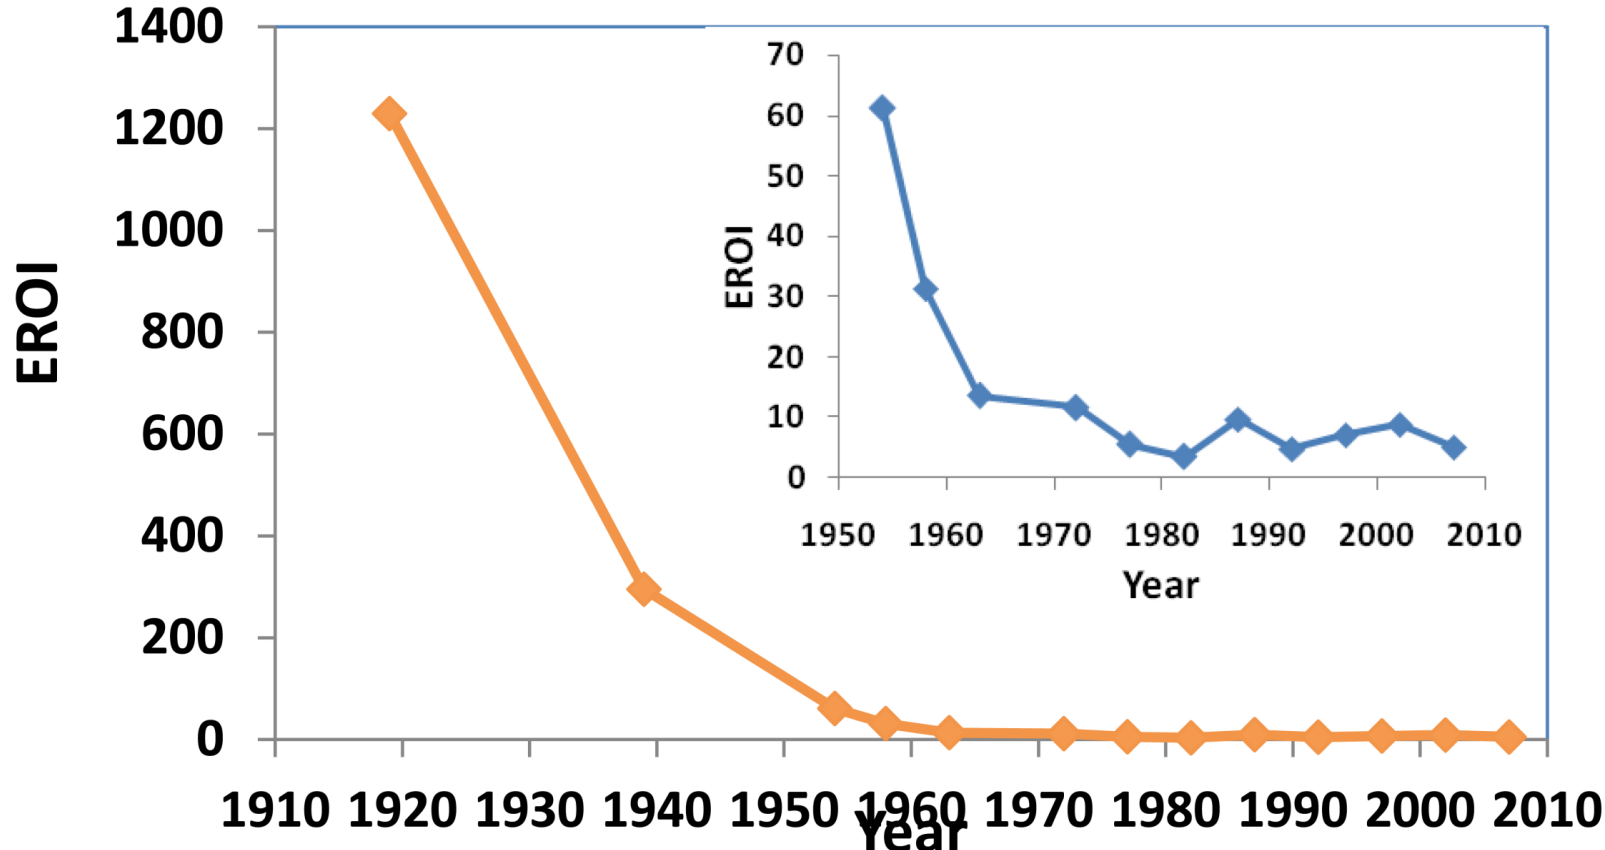
\includegraphics[scale=0.2]{62025-09-23.png}
	\end{center}
	
	On voit ici, lors de la découverte d'un champs c'est souvent les endroits les plus intérressant et les plus facile pour extraire, dès lors on voit que le ROI descend car la facilité d'extraction diminue
    
\end{parag}
\begin{parag}{EROI de la production}
	\begin{center}
	    
	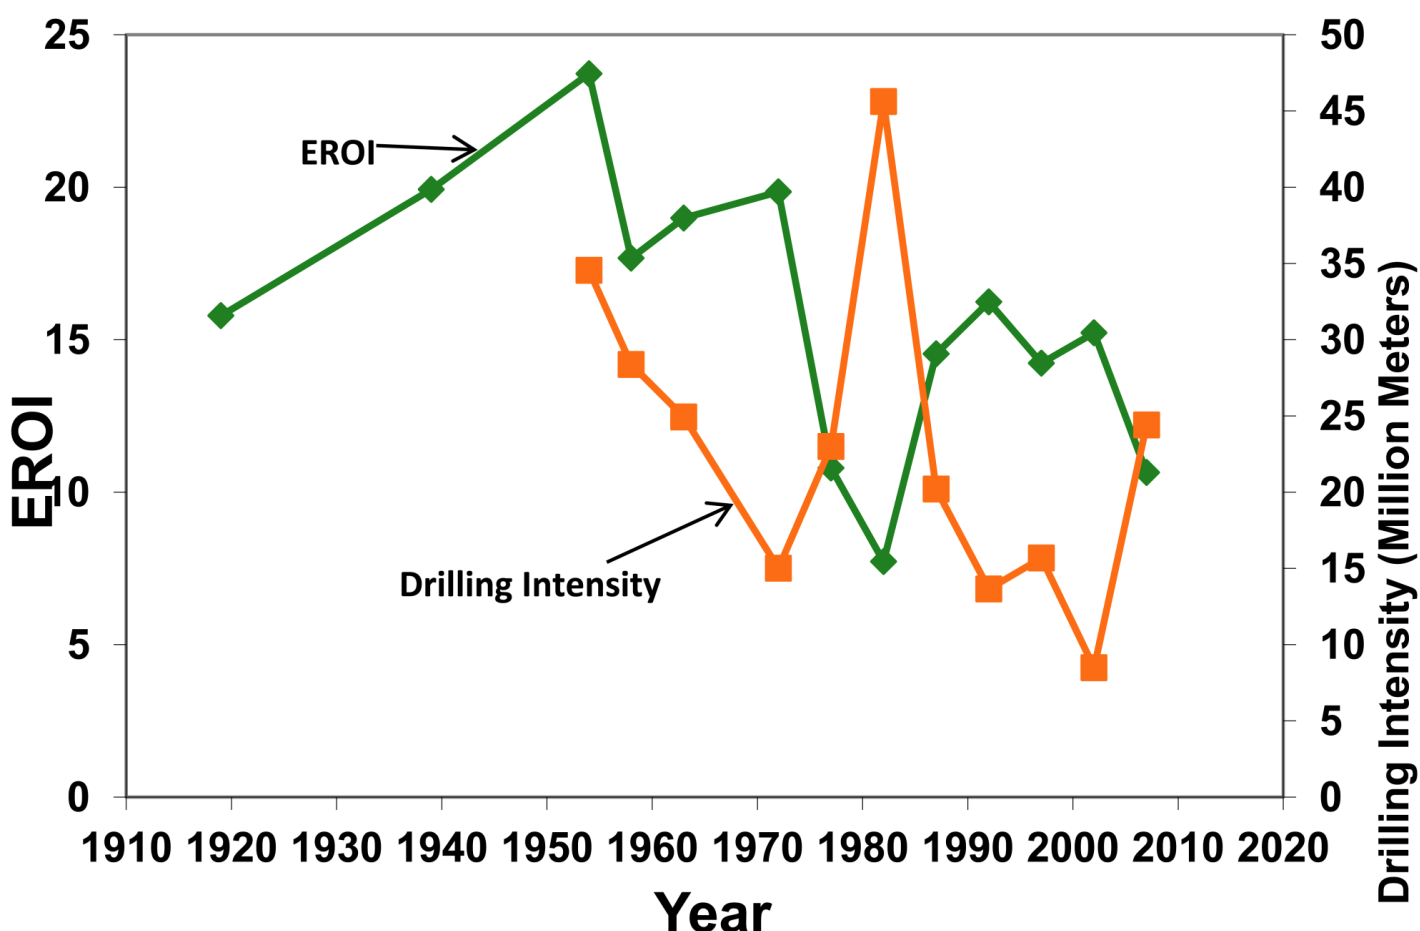
\includegraphics[scale=0.2]{72025-09-23.png}
	\end{center}
	
	Lorsqu'on pompe beaucoup, on va dans des champs qui sont moins bons ce qui donc fait descendre le flux
    
\end{parag}


\subsection{Innovation durable}

\begin{parag}{Différence entre Créativité Innovation Progrès}
	\begin{subparag}{Créativité}
	    Jouer avec ses idées
	\end{subparag}
	\begin{subparag}{Innovation}
	    Generer du profit grâce à sa  créativité $\to$ impact économique
	\end{subparag}
	\begin{subparag}{Progrès}
	    Avoir un impact positif sur la société $\to$ impact sociétal
	\end{subparag}
	\begin{subparag}{Aparté sur l'innovation}
	    Opower (jsp c'est quoi) on voulu faire baisser la consommation d'un habitat. Il voulait le faire en changeant la \important{mentalité des gens} et non la technologie. Par exemple un dashboard de l'argent économisé, ou alors nous faire être sauveur de la planête.\\
	    Le \important{plus rentable}: avoir une compétition entre les voisins, avoir un classement entre les voisins
	\end{subparag}
	\begin{framedremark}
	Par exemple avoir un quartier sans panneau photovoltaique, dès qu'une personne en mets $\to $ effet boule de neige vers le quartier.
	\end{framedremark}
\end{parag}


\begin{parag}{Buisness model canva}
	\begin{center}
    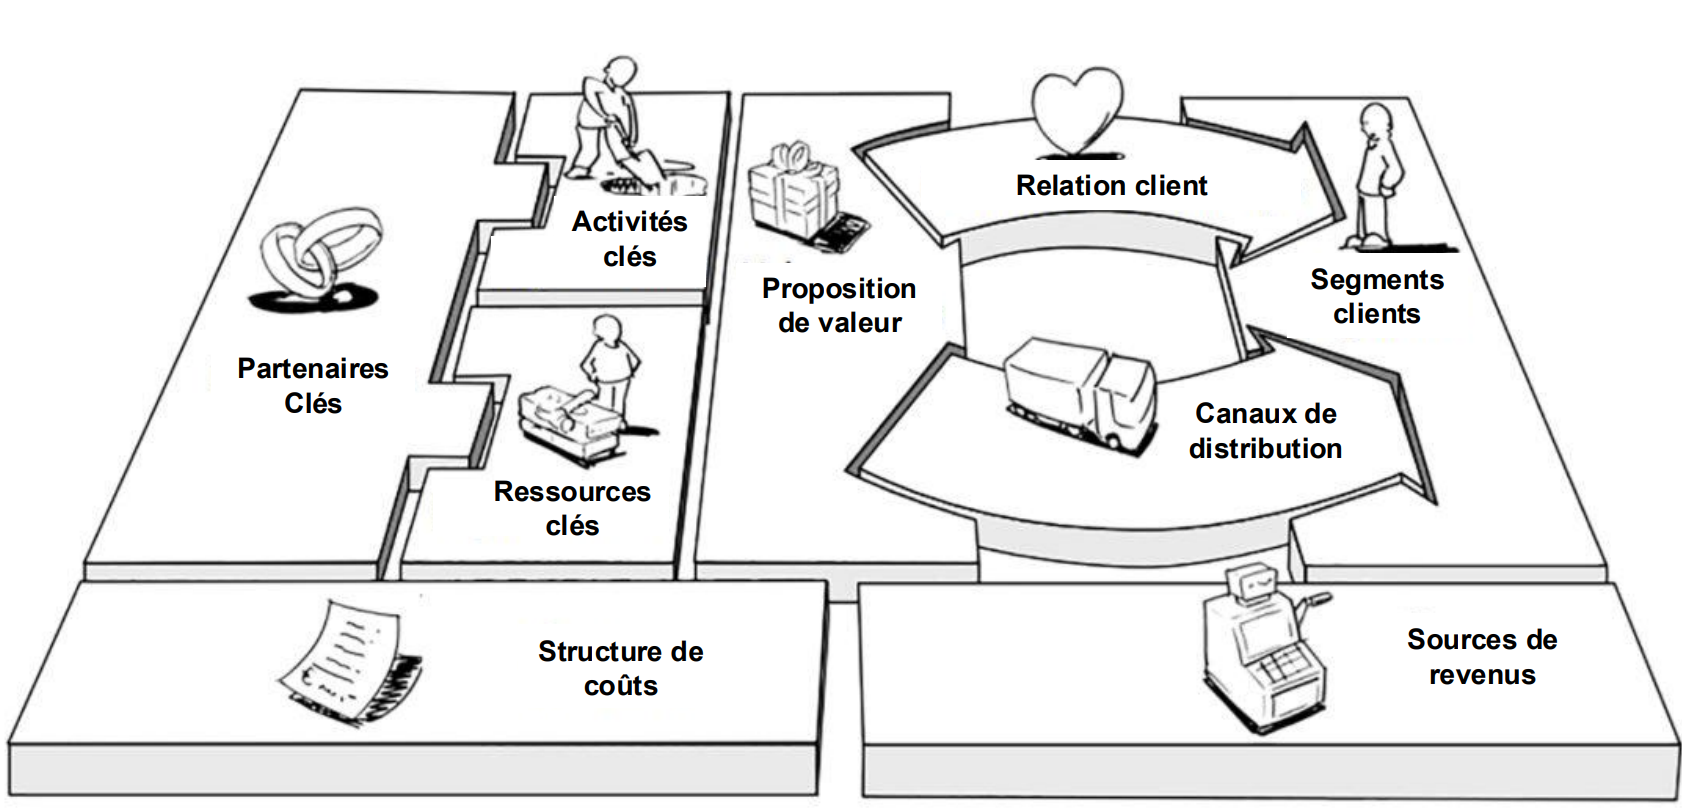
\includegraphics[scale=0.2]{82025-09-23.png}
	\end{center}
	
    \begin{itemize}
	    \item Est ce que c'est faisable?
	    \item Est ce qu'il est viable, revenu $>$ coût?
	    \item Est ce qu'il est désirable? Est ce que des gens veulent acheter votre produit
    \end{itemize}
    
\end{parag}


\begin{parag}{Maslow}
	\begin{center}
    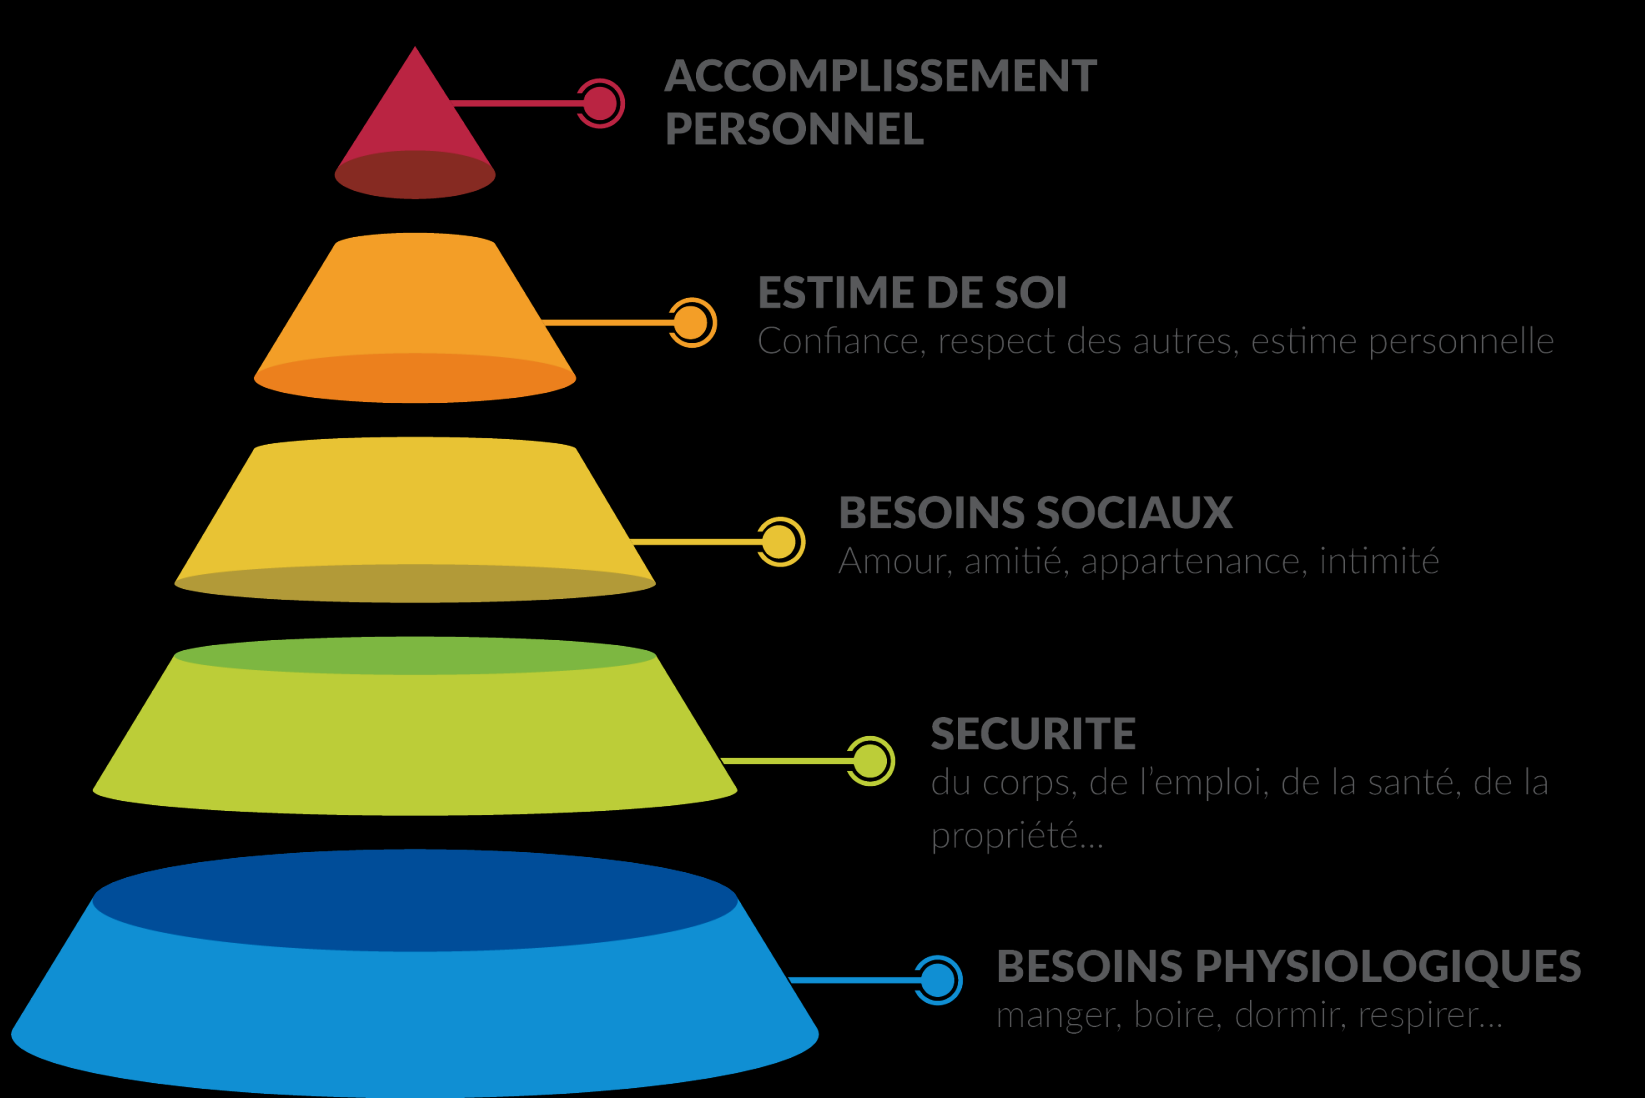
\includegraphics[scale=0.15]{92025-09-23.png}
	\end{center}
	
    Ici on parle des besoins les plus primitifs dans une société jusqu'à ce qui est le moins "nécessaire"\\
    On a plus vraimment de besoin mais plus de désir.\\
    \begin{center}
    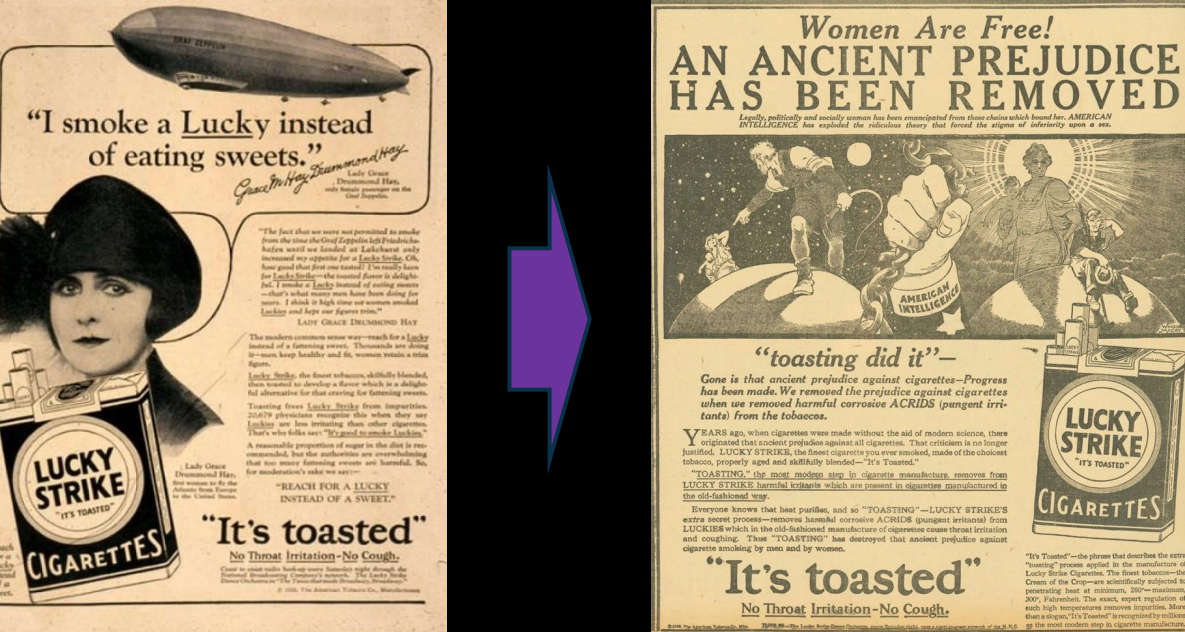
\includegraphics[scale=0.2]{102025-09-23.png}
    \end{center}
    
    Par exemple la cigarette chez les femmes au états unis. Les femmes de l'époques de fumait pas, c'était mal vu. Edward Bernays a alors amené la cigarette comme un produit faisant. La cigarette est aussi devenu un signe de feminisme chez les femmes américaines de l'époque. Grâce à ces deux images la cigarette est devenue populaire aussi chez les femmes.\\
    On voit encore une fois qu'on est passé d'une économie de besoin à une économie de désir.
\end{parag}


\subsection{Robustesse et flexibilité}
\begin{parag}{Prix des technologies}
    Imaginons que nous ayons les quatre intallations éolienne, gaz, nucléaire, hydraulique, quelles sont les problèmes respectifs de chacunes des installations:
    \begin{itemize}
	    \item Eolienne: pas flexible (depend du temps)
	    \item Gaz: flexible
	    \item Nucléaire: flexible, coût si l'on doit arreter
	    \item Hydraulique: très flexible
    \end{itemize}
    Maintenant quelle est le coût:
    \begin{align*} \text{Coût investissement} \approx \frac{\text{investissement initial}}{\text{Energie théorique sur l'ensemble du cycle de vie}} \end{align*}
    
    \begin{align*} \text{Coût carburant ou carbonne} \approx \frac{\text{cout carburant ou carbonne}}{\text{energe generé}} \end{align*}
    \begin{align*} \text{Cout o M}\approx \frac{\text{count annuel des salaires}}{\text{Energie théorique générée durant l'année}} \end{align*}
\end{parag}
\begin{parag}{installations}
	\begin{subparag}{Gaz}
	    Max $1MWh$ chaque période
	\end{subparag}
	\begin{subparag}{Nucléaire}
	    Coût d'arrêt de la centrale
	    \begin{itemize}
		    \item 100CHF
		    \item Max $1MWh$ chaque période
	    \end{itemize}
	    
	\end{subparag}
   \begin{subparag}{Hydro: Accumulation}
	   La production est flexible $1MWh$ stocké (peut produire sur une période seul)
   \end{subparag} 
   \begin{subparag}{Eolien}
       Production intermittente:
       \begin{align*} 17-18MWh \mathspace \mathspace 18-19:0MWh \mathspace \mathspace 19-20:MWh \end{align*}
   \end{subparag}
\end{parag}

\begin{parag}{Coût par installation}
    \begin{center}
    \begin{tabular}{|c|c|c|c|c|}
	    \hline
	    & Eolien & Nucléaire & hydraulique & Gaz \\
	    \hline
	    \hline
	    Investissement  & 38 & 11 & 35 & 9 \\
	    \hline 
	     Démantèlement& 0 & 0 & 0 & 0 \\
	    \hline 
	     Carburant& 0 & 9 & 0 & 46 \\
	    \hline 
	     Carbon& 0 & 0 & 0 & 10 \\
	    \hline 
	     O \& M & 18 & 13 & 5 & 6 \\
	    \hline 
    \end{tabular}
    \end{center}
    
\end{parag}





